\documentclass[11pt,a4paper]{article}
% Preambulo comun de los reportes de Tecnologias Celulares.
% Cada main.tex hace: \documentclass ... % Preambulo comun de los reportes de Tecnologias Celulares.
% Cada main.tex hace: \documentclass ... % Preambulo comun de los reportes de Tecnologias Celulares.
% Cada main.tex hace: \documentclass ... \input{../comun/preambulo.tex}
\usepackage[utf8]{inputenc}
\usepackage[T1]{fontenc}
\usepackage[spanish,mexico]{babel}
\usepackage{graphicx}
\usepackage[margin=2.5cm]{geometry}
\usepackage{amsmath}
\usepackage{amssymb}
\usepackage{booktabs}
\usepackage{tabularx}
\usepackage{array}
\usepackage{float}
\usepackage{setspace}
\usepackage{parskip}
\usepackage{fancyhdr}
\usepackage{textcomp}
\usepackage{xcolor}
\usepackage{caption}
\usepackage{fvextra}
\usepackage[hidelinks]{hyperref}

\onehalfspacing
\setlength{\parskip}{6pt}
\sloppy
\setlength{\emergencystretch}{3em}
\setlength{\headheight}{40pt}
\captionsetup{font=small,labelfont=bf}
\setlength{\tabcolsep}{6pt}

\pagestyle{fancy}
\fancyhf{}
\fancyhead[L]{\includegraphics[width=1cm]{/home/yovick/repos/UAZ-IEI/Assets/UIE.png}}
\fancyhead[R]{\small Comunicaciones Inalámbricas}
\fancyfoot[C]{\thepage}
\renewcommand{\headrulewidth}{0.4pt}

\DefineVerbatimEnvironment{codigo}{Verbatim}{%
  breaklines=true,breakanywhere=true,fontsize=\small,frame=single,
  framesep=3pt,rulecolor=\color{gray!50}}

% Figura centrada con pie: \figura[ancho]{archivo}{leyenda}
\newcommand{\figura}[3][0.85]{%
  \begin{center}
    \includegraphics[width=#1\linewidth]{#2}\\[2pt]
    {\small #3}
  \end{center}}

% Portada: \portada{numero}{titulo de la practica}
\newcommand{\portada}[2]{%
\begin{titlepage}
  \thispagestyle{empty}
  \begin{center}
    \vspace*{1cm}
    \includegraphics[width=4.5cm]{/home/yovick/repos/UAZ-IEI/Assets/uaz.png}
    \vspace{0.8cm}

    {\large Universidad Autónoma de Zacatecas}\\[4pt]
    {\large Unidad Académica de Ingeniería Eléctrica}\\[4pt]
    {\normalsize Ingeniería Electrónica Industrial con especialidad en Telecomunicaciones}

    \vspace{1.8cm}
    {\LARGE\bfseries Práctica #1}\\[10pt]
    {\Large\bfseries #2}
  \end{center}

  \vspace{2.2cm}
  \begin{center}
    \begin{tabular}{rl}
      \textbf{Materia:} & Comunicaciones Inalámbricas\\
      \textbf{Docente:} & Dr. Víktor Iván Rodríguez Abdalá\\
      \textbf{Alumno:}  & Arnold Yovick Ríos Zaldívar\\
      \textbf{Fecha:}   & Noviembre de 2026\\
    \end{tabular}
  \end{center}
  \vfill
\end{titlepage}}

\usepackage[utf8]{inputenc}
\usepackage[T1]{fontenc}
\usepackage[spanish,mexico]{babel}
\usepackage{graphicx}
\usepackage[margin=2.5cm]{geometry}
\usepackage{amsmath}
\usepackage{amssymb}
\usepackage{booktabs}
\usepackage{tabularx}
\usepackage{array}
\usepackage{float}
\usepackage{setspace}
\usepackage{parskip}
\usepackage{fancyhdr}
\usepackage{textcomp}
\usepackage{xcolor}
\usepackage{caption}
\usepackage{fvextra}
\usepackage[hidelinks]{hyperref}

\onehalfspacing
\setlength{\parskip}{6pt}
\sloppy
\setlength{\emergencystretch}{3em}
\setlength{\headheight}{40pt}
\captionsetup{font=small,labelfont=bf}
\setlength{\tabcolsep}{6pt}

\pagestyle{fancy}
\fancyhf{}
\fancyhead[L]{\includegraphics[width=1cm]{/home/yovick/repos/UAZ-IEI/Assets/UIE.png}}
\fancyhead[R]{\small Comunicaciones Inalámbricas}
\fancyfoot[C]{\thepage}
\renewcommand{\headrulewidth}{0.4pt}

\DefineVerbatimEnvironment{codigo}{Verbatim}{%
  breaklines=true,breakanywhere=true,fontsize=\small,frame=single,
  framesep=3pt,rulecolor=\color{gray!50}}

% Figura centrada con pie: \figura[ancho]{archivo}{leyenda}
\newcommand{\figura}[3][0.85]{%
  \begin{center}
    \includegraphics[width=#1\linewidth]{#2}\\[2pt]
    {\small #3}
  \end{center}}

% Portada: \portada{numero}{titulo de la practica}
\newcommand{\portada}[2]{%
\begin{titlepage}
  \thispagestyle{empty}
  \begin{center}
    \vspace*{1cm}
    \includegraphics[width=4.5cm]{/home/yovick/repos/UAZ-IEI/Assets/uaz.png}
    \vspace{0.8cm}

    {\large Universidad Autónoma de Zacatecas}\\[4pt]
    {\large Unidad Académica de Ingeniería Eléctrica}\\[4pt]
    {\normalsize Ingeniería Electrónica Industrial con especialidad en Telecomunicaciones}

    \vspace{1.8cm}
    {\LARGE\bfseries Práctica #1}\\[10pt]
    {\Large\bfseries #2}
  \end{center}

  \vspace{2.2cm}
  \begin{center}
    \begin{tabular}{rl}
      \textbf{Materia:} & Comunicaciones Inalámbricas\\
      \textbf{Docente:} & Dr. Víktor Iván Rodríguez Abdalá\\
      \textbf{Alumno:}  & Arnold Yovick Ríos Zaldívar\\
      \textbf{Fecha:}   & Noviembre de 2026\\
    \end{tabular}
  \end{center}
  \vfill
\end{titlepage}}

\usepackage[utf8]{inputenc}
\usepackage[T1]{fontenc}
\usepackage[spanish,mexico]{babel}
\usepackage{graphicx}
\usepackage[margin=2.5cm]{geometry}
\usepackage{amsmath}
\usepackage{amssymb}
\usepackage{booktabs}
\usepackage{tabularx}
\usepackage{array}
\usepackage{float}
\usepackage{setspace}
\usepackage{parskip}
\usepackage{fancyhdr}
\usepackage{textcomp}
\usepackage{xcolor}
\usepackage{caption}
\usepackage{fvextra}
\usepackage[hidelinks]{hyperref}

\onehalfspacing
\setlength{\parskip}{6pt}
\sloppy
\setlength{\emergencystretch}{3em}
\setlength{\headheight}{40pt}
\captionsetup{font=small,labelfont=bf}
\setlength{\tabcolsep}{6pt}

\pagestyle{fancy}
\fancyhf{}
\fancyhead[L]{\includegraphics[width=1cm]{/home/yovick/repos/UAZ-IEI/Assets/UIE.png}}
\fancyhead[R]{\small Comunicaciones Inalámbricas}
\fancyfoot[C]{\thepage}
\renewcommand{\headrulewidth}{0.4pt}

\DefineVerbatimEnvironment{codigo}{Verbatim}{%
  breaklines=true,breakanywhere=true,fontsize=\small,frame=single,
  framesep=3pt,rulecolor=\color{gray!50}}

% Figura centrada con pie: \figura[ancho]{archivo}{leyenda}
\newcommand{\figura}[3][0.85]{%
  \begin{center}
    \includegraphics[width=#1\linewidth]{#2}\\[2pt]
    {\small #3}
  \end{center}}

% Portada: \portada{numero}{titulo de la practica}
\newcommand{\portada}[2]{%
\begin{titlepage}
  \thispagestyle{empty}
  \begin{center}
    \vspace*{1cm}
    \includegraphics[width=4.5cm]{/home/yovick/repos/UAZ-IEI/Assets/uaz.png}
    \vspace{0.8cm}

    {\large Universidad Autónoma de Zacatecas}\\[4pt]
    {\large Unidad Académica de Ingeniería Eléctrica}\\[4pt]
    {\normalsize Ingeniería Electrónica Industrial con especialidad en Telecomunicaciones}

    \vspace{1.8cm}
    {\LARGE\bfseries Práctica #1}\\[10pt]
    {\Large\bfseries #2}
  \end{center}

  \vspace{2.2cm}
  \begin{center}
    \begin{tabular}{rl}
      \textbf{Materia:} & Comunicaciones Inalámbricas\\
      \textbf{Docente:} & Dr. Víktor Iván Rodríguez Abdalá\\
      \textbf{Alumno:}  & Arnold Yovick Ríos Zaldívar\\
      \textbf{Fecha:}   & Noviembre de 2026\\
    \end{tabular}
  \end{center}
  \vfill
\end{titlepage}}


\graphicspath{{figs/}}

\newcommand{\listado}[1]{%
  \VerbatimInput[fontsize=\scriptsize,breaklines=true,breakanywhere=true,
    frame=single,framesep=2pt,rulecolor=\color{gray!50},numbers=left,
    numbersep=4pt]{#1}}

\begin{document}
\thispagestyle{empty}

% --------------------------------------------------------------- encabezado
\begin{center}
  \includegraphics[width=2.6cm]{/home/yovick/repos/UAZ-IEI/Assets/uaz.png}\\[2mm]
  {\large Universidad Autónoma de Zacatecas}\\
  {\normalsize Unidad Académica de Ingeniería Eléctrica}\\
  {\normalsize Ingeniería Electrónica Industrial con especialidad en Telecomunicaciones}\\[6mm]
  {\LARGE\bfseries Tarea 1}\\[2mm]
  {\large Transmisión a través de canales inalámbricos}\\[5mm]
  {\small
  \begin{tabular}{rl}
    \textbf{Materia:}   & Comunicaciones Inalámbricas\\
    \textbf{Docente:}   & Dr. Víktor Iván Rodríguez Abdalá\\
    \textbf{Alumno:}    & Arnold Yovick Ríos Zaldívar\\
    \textbf{Matrícula:} & 35167151 \quad \textbf{Grupo:} VII\\
    \textbf{Fecha:}     & Noviembre de 2026\\
  \end{tabular}}
\end{center}

\vspace{2mm}

Los 11 problemas se resolvieron con \texttt{tarea1.py}. Los canales son de
desvanecimiento Rayleigh lento y las señales binarias se simulan con $E_b=1$ y
ruido complejo de varianza $N_0$. Las figuras y los números se regeneran con
\texttt{python3 tarea1.py}.

% ------------------------------------------------------------- problema 1
\section*{Problema 1: variables Rayleigh con $\sigma^2=1,5,10$}

Se generaron 2000 muestras $r=\sigma\sqrt{-2\ln u}$ para cada $\sigma^2$ y se
comparó el histograma con la PDF $f(r)=\frac{r}{\sigma^2}e^{-r^2/2\sigma^2}$.
Las medias muestrales fueron 1.25, 6.35 y 12.34, frente a las teóricas
$\sigma\sqrt{\pi/2}=1.25$, 6.27 y 12.53.

\begin{figure}[H]
  \centering
  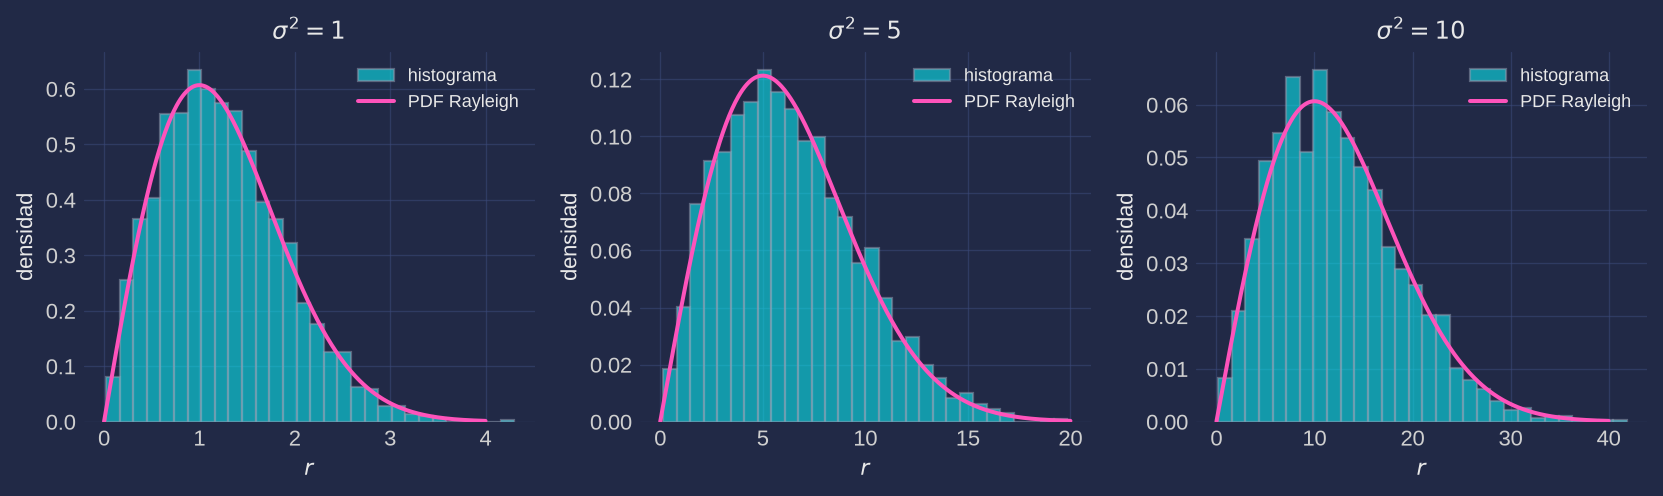
\includegraphics[width=\linewidth]{p1_rayleigh.png}
  \caption{Histogramas de las variables Rayleigh y su PDF teórica.}
\end{figure}

% ------------------------------------------------------------- problema 2
\section*{Problema 2: taps con un filtro de un polo}

Con $H(z)=\frac{1-p}{1-pz^{-1}}$ la recursión es
$c_n=pc_{n-1}+(1-p)w_n$, con $w_n$ blanco complejo. Para $p=0.9$ la varianza
de $c_n$ es 0.046 y la autocorrelación a un retardo 0.889; para $p=0.99$ son
0.0040 y 0.988. El polo cercano a 1 concentra el espectro y hace que los taps
varíen mucho más lento.

\begin{figure}[H]
  \centering
  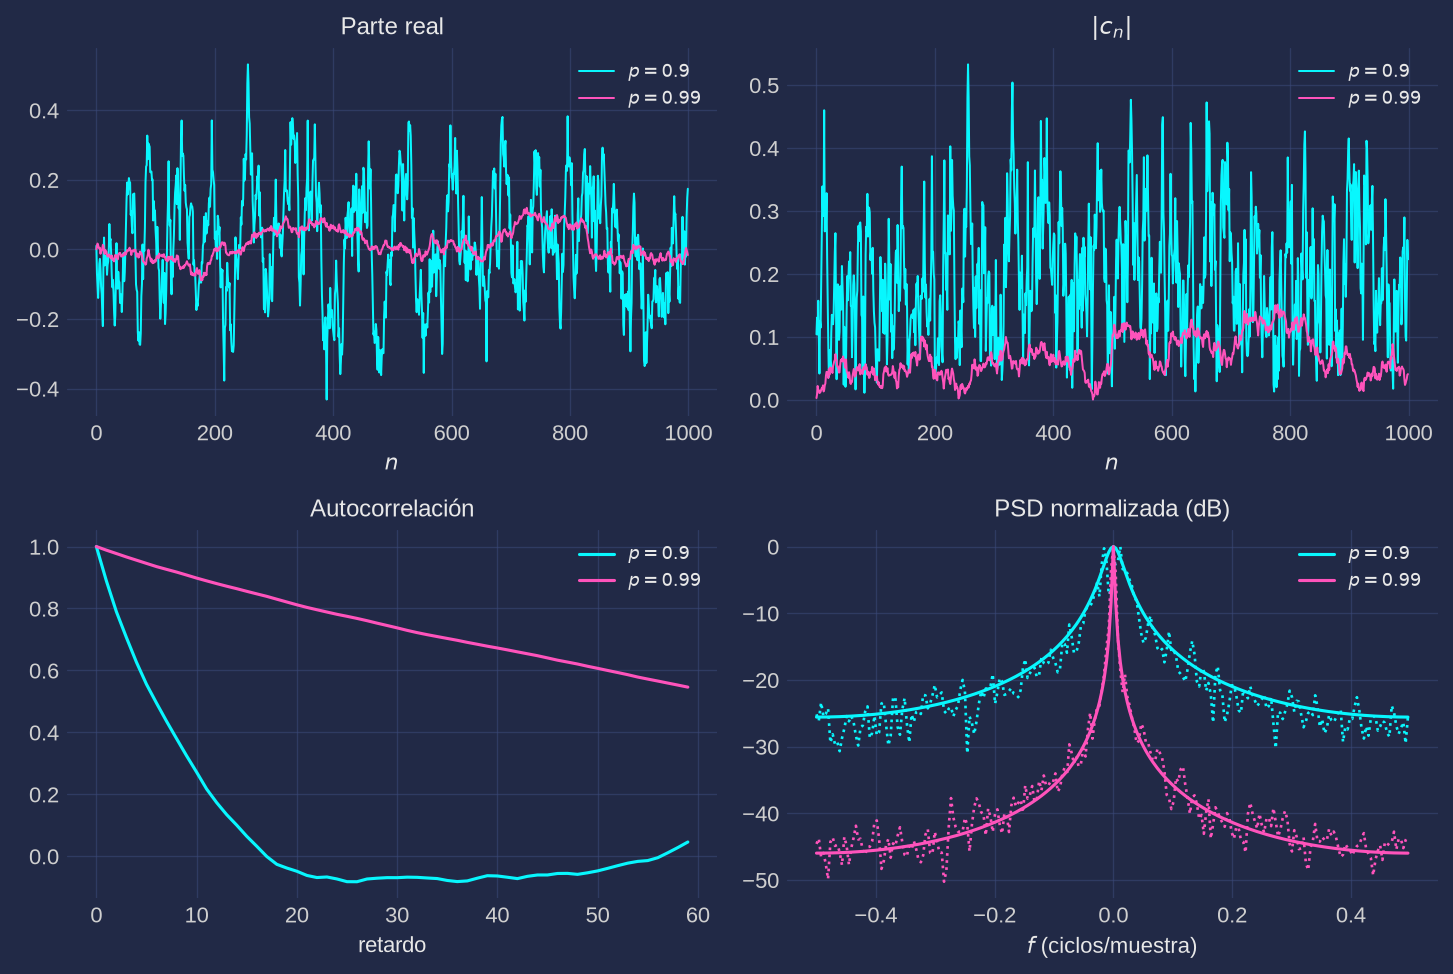
\includegraphics[width=0.92\linewidth]{p2_taps.png}
  \caption{Coecientes de tap, autocorrelación y PSD para $p=0.9$ y $p=0.99$
  (puntos: estimación de Welch; línea: $|H|^2$).}
\end{figure}

% ------------------------------------------------------------- problema 3
\section*{Problema 3: espectro Doppler de Jakes}

A $v=200$ km/h y $f_c=1$ GHz, la frecuencia Doppler máxima es
\begin{equation}
  f_m=\frac{vf_c}{c}=\frac{55.56\times10^9}{3\times10^8}=185.2\ \text{Hz},
\end{equation}
y el espectro es $S(f)=1/(\pi f_m\sqrt{1-(f/f_m)^2})$ para $|f|\le f_m$.

\begin{figure}[H]
  \centering
  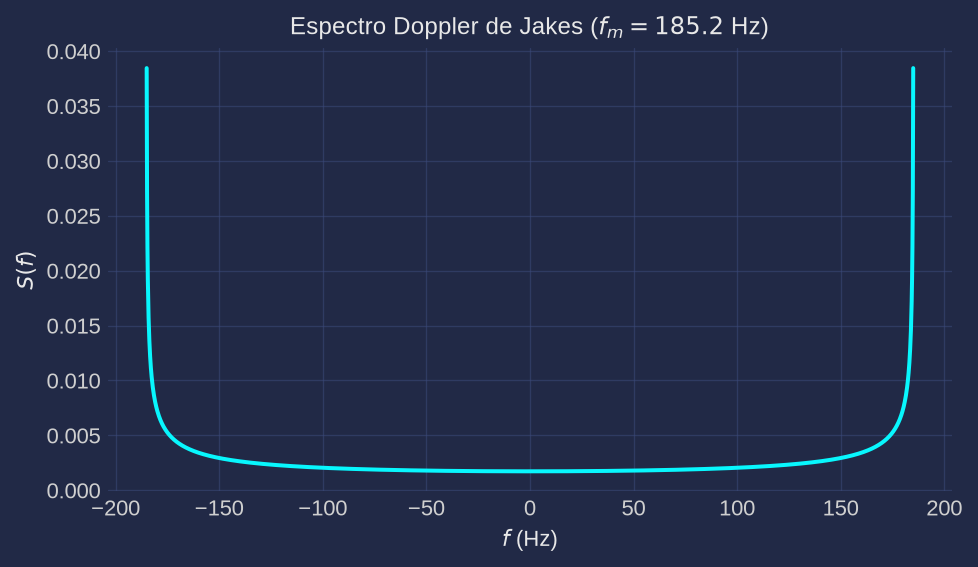
\includegraphics[width=0.7\linewidth]{p3_jakes.png}
  \caption{Espectro Doppler de Jakes para $f_m=185.2$ Hz.}
\end{figure}

% ---------------------------------------------------------- problemas 4 a 6
\section*{Problemas 4 a 6: señalización binaria en Rayleigh}

Para señales ortogonales con detección no coherente (ley cuadrada),
$P_e=1/(2+\bar\rho_b)$. Para OOK coherente con umbral $|c|^2\sqrt{E_b}/2$,
$P_e=\frac12(1-\sqrt{\bar\rho_b/(\bar\rho_b+4)})$. Con diversidad $D=3$ y
combinación de ley cuadrada, la asíntota es $P_2\approx K_D/\bar\rho^3$, con
$K_3=10$ y $\bar\rho=\bar\rho_b/3$.

La simulación sigue las tres curvas: a 10 dB las BER medidas son 0.083, 0.077
y 0.049, y a 20 dB 0.0092, 0.0099 y $1.6\times10^{-4}$.

\begin{figure}[H]
  \centering
  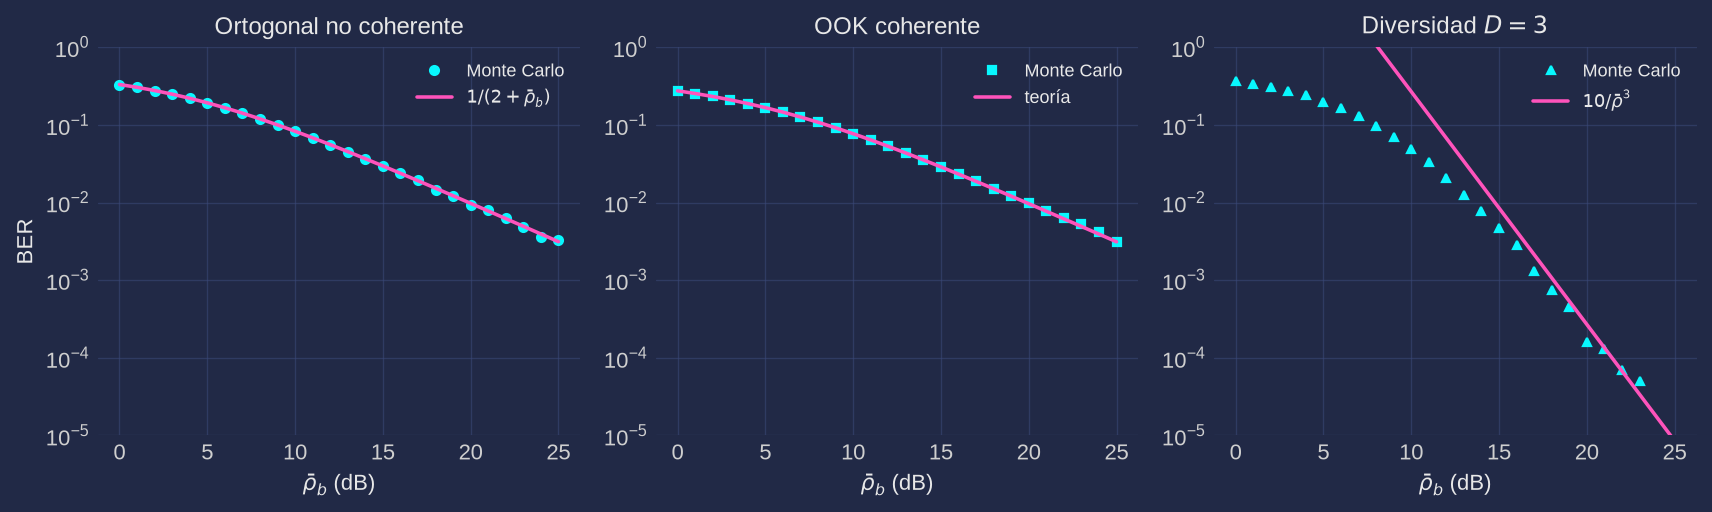
\includegraphics[width=\linewidth]{p456_binarias.png}
  \caption{Ortogonal no coherente, OOK y diversidad $D=3$: Monte Carlo contra
  teoría.}
\end{figure}

% ---------------------------------------------------------- problemas 7 y 8
\section*{Problemas 7 y 8: receptor RAKE de dos trayectorias}

Con señales ortogonales y estimación perfecta del canal, el RAKE combina cada
señal con $\sum_k c_k^*r_{ik}$ y decide por la mayor parte real. Para dos rayos
iguales, la asíntota es $P_2\approx 3/(2\bar\rho)^2=3/\bar\rho_b^2$; si la
primera trayectoria tiene el doble de potencia que la segunda,
$P_2\approx 3/(4\bar\rho_1\bar\rho_2)=27/(8\bar\rho_b^2)$.

A 20 dB se midieron $3.0\times10^{-4}$ y $3.2\times10^{-4}$, en acuerdo con
$3.0\times10^{-4}$ y $3.4\times10^{-4}$.

\begin{figure}[H]
  \centering
  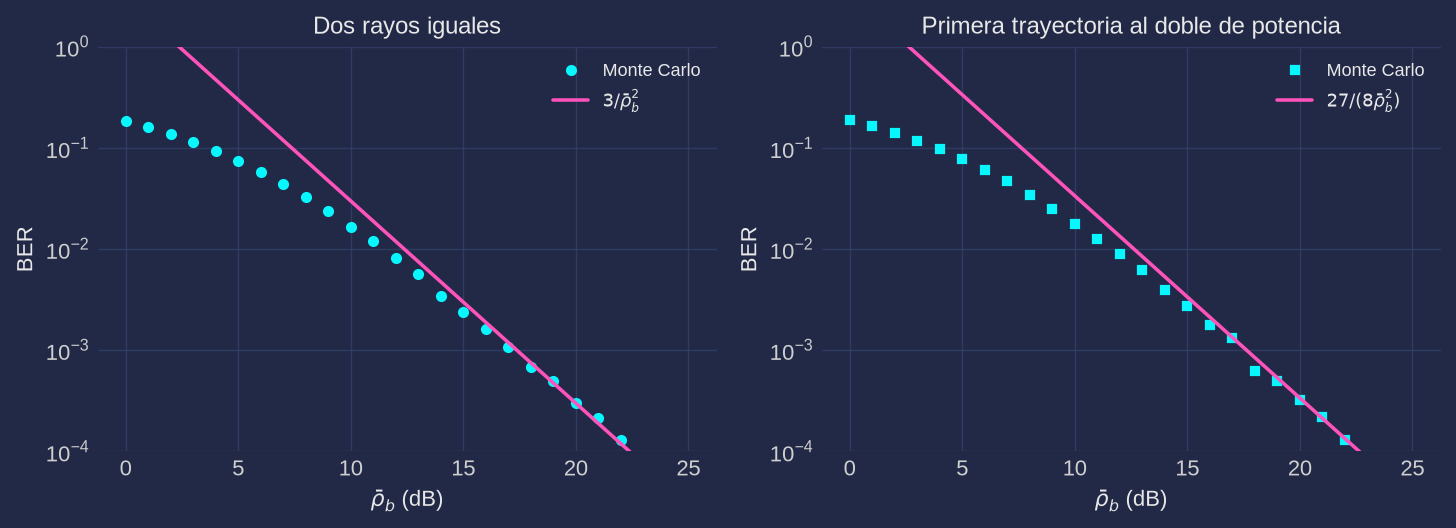
\includegraphics[width=\linewidth]{p78_rake.png}
  \caption{RAKE de dos trayectorias: rayos iguales y primera trayectoria al
  doble de potencia.}
\end{figure}

% ------------------------------------------------------------- problema 9
\section*{Problema 9: diseño OFDM}

Con $W=800$ kHz, $T_m=10\,\mu$s y $B_d=10$ Hz, se elige $T=10T_m=100\,\mu$s
para que el prefijo cíclico cueste cuando mucho el 10\% del símbolo. Entonces
$\Delta f=1/T=10$ kHz, $N=W/\Delta f=80$ subcanales, $T_{ct}=1/B_d=0.1$ s y
$B_{cb}=1/T_m=100$ kHz. Como $T\ll T_{ct}$, el canal es lento dentro del
símbolo, y como $W\gg B_{cb}$, es selectivo en frecuencia. La diversidad
máxima por frecuencia es $W/B_{cb}=8$ subcanales independientes; la tasa útil
es $N/T=800$ ksímbolos/s sin diversidad.

% ------------------------------------------------------------ problemas 10 y 11
\section*{Problemas 10 y 11}

De (41), $T_m\ll T\ll T_{ct}=1/B_d$. Dividiendo entre $T_m$ y usando
$T\ll1/B_d$,
\begin{equation}
  T_m\ll T\ll \frac{1}{B_d}\;\Longrightarrow\;T_mB_d\ll1 ,
\end{equation}
que es la condición de canal sin esparcimiento (variación lenta frente a la
dispersión).

De (41) y (42), $W\gg B_{cb}=1/T_m$ y $T\gg T_m$, de modo que
\begin{equation}
  W\gg\frac{1}{T_m}\gg\frac{1}{T}\;\Longrightarrow\;TW\gg1 .
\end{equation}

% ------------------------------------------------------------- conclusiones
\section*{Conclusiones}

\begin{itemize}
  \item El histograma Rayleigh coincide con la PDF para $\sigma^2=1,5,10$;
        la media escala como $\sigma\sqrt{\pi/2}$.
  \item Un polo cercano a 1 ensancha la correlación temporal y estrecha el
        espectro Doppler, que es el efecto que se busca en el modelo de taps.
  \item A 200 km/h y 1 GHz, $f_m=185$ Hz.
  \item La detección no coherente, el OOK y la diversidad siguen las curvas
        teóricas; el RAKE alcanza diversidad 2 y la trayectoria fuerte mejora
        apenas 0.5 dB la asíntota.
  \item El diseño OFDM con $T=100\,\mu$s da 80 subcanales y hasta 8 ramas de
        diversidad en frecuencia para $W=800$ kHz.
\end{itemize}

% ------------------------------------------------------------------ codigo
\appendix
\section*{Código}
\listado{tarea1.py}

\end{document}
